\section{Prediction}
The goal of the task is to fit a prediction model that will predict the final position of a given cyclist in a race, discriminating those cyclists whose placement is in the top 20 (class 1) positions from the others (class 0). To pursue this goal, we revamped the data cleaning and feature engineering tasks to prepare the races dataset for classification.

\subsection{Data Cleaning}
First, we eliminated those stages associated with a null \textit{climb\_total} or \textit{profile} feature value. Since we used those features to engineer new ones, we avoided dealing with null values. This operation dropped $180'556$ of $589'616$ total rows. On a professor's advice, we also eliminated the stages with less than 25 participants to avoid non-representative data, as smaller group sizes could disproportionately affect the distinction between the top 20 cyclists and non-top 20 cyclists. To facilitate this operation, we counted how many cyclists each stage had adding this information to the dataset.

\subsection{Feature Engineering}
We engineered some new features the task can rely on. Below you can find a detailed overview. \\

\noindent
\textbf{top\_20}: this feature represents the classification label: 1 if the position associated with a cyclist is smaller or equal to 20 and 0 otherwise.\\ \\
Some basic statistics run on this column made us aware of an important dataset-related thing: the unbalance. Class 0 represents 87\% of the entire dataset while class 1 only has 13\%. In the next section, we will consider some of the issues related to this problem. \\

\noindent
\textbf{cyclist\_level}: this feature quantifies the level of a cyclist considering all the placements until the stage for which we are calculating the feature. This feature is calculated using the method described in \autoref{sec:feat_eng}. \\

\noindent
\textbf{cyclist\_experience}: this feature counts the number of stages a cyclist participated in until the stage for which we calculate the feature. \\

\noindent
\textbf{avg\_relative\_position}: this feature represents the average positioning of the cyclist and it's calculated as described in \autoref{sec:feat_eng}, with the distinction that it is computed up to, but excluding the current stage. \\

\noindent
\textbf{avg\_relative\_position\_profile}: this feature expresses the average relative position reached by a cyclist in a specific race's profile until the stage for which we calculate the feature. \\

\noindent
\textbf{rel\_position\_length}: this feature expresses the relative position reached by a cyclist in a particular class of race's length i.e. 0 (short), 1 (medium), 2 (long) until the stage for which we are calculating the feature. \\

\noindent
\textbf{rel\_position\_climb}: this feature represents the average relative position reached by a cyclist in a race taking into account a particular race climb until the stage for which we are calculating the feature. To do this we defined three classes of climbs: 0 (flat/low climb), 1 (hilly/medium climb), and 2 (mountainous/high climb). \\

\noindent
\textbf{avg\_cyclist\_level}: this feature replaces the \textit{startlist\_quality} feature. It expresses the same idea but is calculated using our engineered feature \textit{cyclist\_level}.\\

\noindent
\textbf{position\_entropy}: this feature expresses the entropy of a cyclist's position in all the stages until the one for which the feature is computed.\\

\noindent
\textbf{top\_20\_entropy}: same reasoning as the previous feature but related to the top 20: the higher the entropy the more unpredictable the positioning in the first position is. \\

\noindent At the end of the process, there were 32 total columns in the dataset.

\subsubsection{Feature Correlation}
We analyzed correlations before splitting the dataset into training, validation, and test sets.

\noindent As one can see from the Figure \ref{fig:class-correlations} there are some high-correlated features, which are: \textit{climb\_total}, \textit{profile}, \textit{cyclist\_age}, \textit{cyclist\_level}, \textit{cyclist\_experience}, \textit{relative\_position}, \textit{avg\_relative\_position}, \\ \textit{cyclist\_experience\_profile}, \textit{cyclist\_experience\_length}, \textit{avg\_rel\_position\_climb}, \textit{position\_entropy}.

Most correlations were expected since they occur between features used to engineer others. Of course, since we cannot deal with highly correlated features during the classification, we decided to select only a subset of non-correlated features.


\subsection{The imbalance dataset problem}
\label{subsec:imbalancing}
Building a binary classifier on an imbalanced dataset like ours poses significant challenges. The dataset reflects a real scenario, with only a small percentage of cyclists in the top 20, leading to potential classifier bias toward the majority class, which comprises 84\% of the data. Simple models risk predicting not-top 20 for all inputs, failing to capture minority class patterns and generalize effectively, which may lead to overfitting. Misleading metrics like accuracy emphasize the dominance of the majority class, making alternatives like the f1-score more suitable. Considering the significant class imbalance in the dataset and the critical importance of class 1 to class 0, we chose to optimize the models based on the standard F1-score.

\begin{figure}[H]
    \centering
    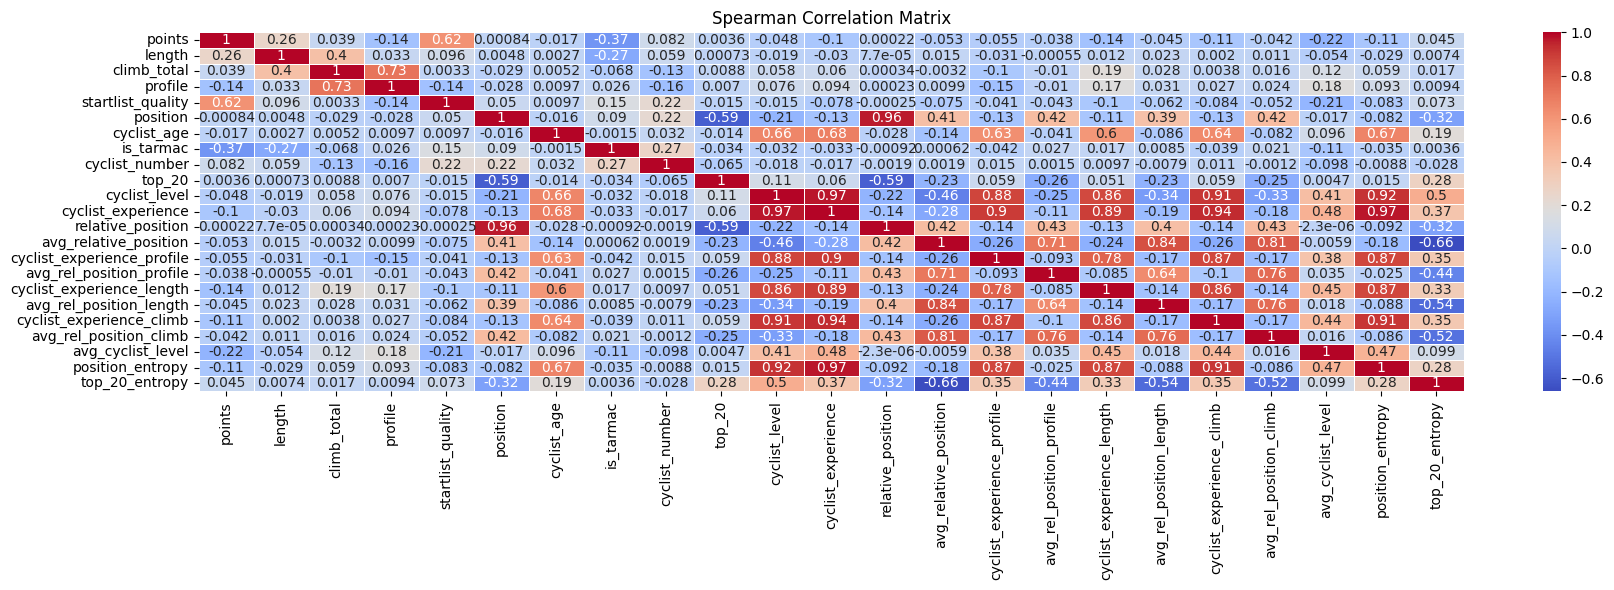
\includegraphics[width=0.88\linewidth]{images/CLASSIFICATION/correlations.png}
    \caption{\small Correlation between numerical features during feature engineering process for the classification}
    \label{fig:class-correlations}
\end{figure}




\subsection{Task Complexity and Classification Challenges}
\label{subsec:extra_analysis}
The extra analysis (\enquote{\texttt{TASK\_5/extra\_analyis.ipynb}}) highlights the inherent challenges of the classification task, emphasizing that the dataset and the nature of the problem make achieving reliable predictions difficult. First, the extra analysis reveals overlapping class distributions in 2D and 3D feature spaces, further complicating classification. Mutual information values for features are low, indicating weak predictive power. To further investigate, we shuffled the labels to simulate a random dataset and compared the results with our model's performance. The model’s slightly better performance suggests weak but present patterns that are difficult to capture effectively.
Further complicating the task is the strategic nature of cycling, which impacts the dataset's structure and predictive potential. In races like the Giro d’Italia, overall success is determined by accumulated time rather than consistent stage victories. Cyclists aiming for the general classification often adopt strategies such as prioritizing minimal time losses in crucial stages while finishing in lower positions in others, sometimes as far back as 100th place, to conserve energy or focus on more critical stages in tightly scheduled races. These strategic decisions, influenced by factors such as team support, energy conservation, and tactical positioning, introduce variability that makes stage-level results context-dependent. Additionally, variables like weather, terrain, and race dynamics are absent from the dataset and add unpredictability, further complicating the task.
To validate this, we analyzed cyclists who achieved victories or top finishes in prestigious races like the Giro d’Italia and the Tour de France. Despite their overall success, these cyclists often recorded significantly low positions in individual stages, underscoring the challenge of relying solely on stage-level results. While not a rigorous statistical demonstration, this analysis supports the conclusion that the task, as formulated, struggles to encapsulate the complexities of cycling, making accurate classification inherently difficult.

\subsection{Our approach to the task}
We employed a multi-model training approach, with the analysis focused on: Naive-Bayes, Logistic Regression, K-NN, Decision Tree, SVM, Random Forest, Gradient Boosting Machine, Neural Network, and Rule-Based Classifier. We optimized each model using hyperparameter searches, various feature combinations, and sampling strategies. After testing various feature subsets, we selected \textit{climb\_total}, \textit{cyclist\_age}, \textit{cyclist\_level}, \textit{cyclist\_experience}, \textit{avg\_relative\_position}, \textit{position\_entropy}, and \textit{top\_20\_entropy} as they give better results. Categorical features were excluded to ensure a fair comparison across models, as many do not support them. Their removal also did not alter the analysis.

Data was split into training and test sets according to the task, shuffled to avoid chronological bias, and trained using 5-fold cross-validation for reliable results. A random grid search with 50 iterations allowed optimized hyperparameters' search, except for Naive-Bayes, for which we performed a complete grid search (because it has only one parameter). To address the class imbalance problem, we decided to compare the model's performance first without any sampling strategy, and then with oversampling, undersampling, or SMOTETomek. Some models (e.g., Rule-Based Classifier and SVM) faced time constraints so we excluded them from the trials (SVM) or we tested just a subset of approaches (RIPPER).

For evaluation, we selected the strategy with the highest f1-score on the validation set and, for the f1-score, we used the ROC AUC to compare results. Comprehensive metrics including Sensitivity, Specificity, Accuracy, Precision, Recall, ROC-AUC, and f1, were calculated for the training, validation, and test sets to evaluate performance.

\subsection{Models Results Overview}
Models were ranked by complexity, starting with the baseline. Results are reported in \autoref{tab:results}.  
The best \textbf{Naive Bayes} used SMOTETomek, with a variance of 0.003, achieving an f1-score of 0.347. 
The best \textbf{Logistic Regression} attempt used SMOTETomek sampling, a regularization of 0.01, no penalty, 0.1 tolerance, 2000 as max iterations, and Sag as the solver, achieving an average f1-score of 0.373 on validation. The \textbf{K-NN Classifier} with undersampling performed slightly better, achieving a 0.397 f1-score, but its configuration details were unavailable due to training time constraints. The K-NN model is the only one exhibiting significant overfitting, achieving near-perfect performance on the training set, but experiencing a sharp decline across all metrics on validation and test sets.

The \textbf{Rule-Based Classifier}, specifically the RIPPER model, achieved an f1-score of 0.377 with undersampling, using a prune size of 0.2, a termination allowance of 0.3, and 4 optimization iterations. The model extracted five rules based solely on \textit{top\_20\_entropy}, but they lacked practical utility, as they defined only a lower entropy bound, promoting high variability. Instead, we want the converse behavior.  

Concerning \textbf{Neural Network}, it performed best with undersampling, achieving an f1-score of 0.392. The optimal configuration found with grid search had three layers with 50, 30, and 10 units, a regularization term of 0.001, a batch size of 128, and a tolerance of 0.001 to halt training when no further improvements are observed.

For tree-based models, the optimal \textbf{Decision Tree} employed SMOTETomek sampling, balanced class weights, a maximum depth of 5, `log2` as the criterion for selecting the maximum number of features at each split, an impurity decrease threshold of 0.0004, and specific constraints on sample splits and leaf sizes. It achieved an f1-score of 0.376 on the validation set. From the decision tree plot and its native feature importance, it is evident that the model primarily focused on two features: \textit{top\_20\_entropy} and \textit{avg\_relative\_position}.  
The best \textbf{Random Forest} attempt used SMOTETomek as sampling, sampling 60\% of the features per tree to reduce overfitting while maintaining diversity. The `subsample=0.2` parameter limited each tree to fit on 20\% of the training samples, enhancing model robustness. With a `max\_depth=8`, the trees were constrained to prevent over-complexity. The ensemble consists of 50 trained trees and achieves an f1-score of 0.371, emphasizing the same key features as the Decision Tree.  
The \textbf{Gradient Boosting Machine} achieved an f1-score of 0.412 when using SMOTETomek as a resampling strategy. The thorough analysis of this outcome is presented in \autoref{subsubsec:best_model}.


%RESULT TABLE
\begin{table}[H]
    \centering
    \scriptsize
    \begin{tabular}{p{2.0cm}ccccccc}
    \toprule
    \textbf{Model} & \textbf{Accuracy} & \textbf{Sensitivity} & \textbf{Specificity} & \textbf{Precision} & \textbf{Recall} & \textbf{f1-score} & \textbf{ROC AUC} \\
    \midrule
    \textbf{NB} 
      & 0.781$\pm$0.001
      & 0.439$\pm$0.003
      & 0.833$\pm$0.001
      & 0.287$\pm$0.001
      & 0.439$\pm$0.003
      & 0.347$\pm$0.002
      & 0.717$\pm$0.002 \\
    \textbf{Logistic Reg.} 
      & 0.799$\pm$0.004
      & 0.451$\pm$0.014
      & 0.852$\pm$0.006
      & 0.318$\pm$0.004
      & 0.451$\pm$0.014
      & 0.373$\pm$0.005
      & 0.746$\pm$0.001 \\
    \textbf{KNN}
      & 0.843$\pm$0.001
      & 0.389$\pm$0.006
      & 0.913$\pm$0.001
      & 0.405$\pm$0.004
      & 0.389$\pm$0.006
      & 0.397$\pm$0.005
      & 0.763$\pm$0.001 \\
    \textbf{RIPPER}
      & 0.747$\pm$0.025
      & 0.575$\pm$0.033
      & 0.773$\pm$0.032
      & 0.282$\pm$0.022
      & 0.575$\pm$0.033
      & 0.377$\pm$0.020
      & 0.687$\pm$0.014 \\
    \textbf{NN}
      & 0.714$\pm$0.004
      & 0.695$\pm$0.007
      & 0.717$\pm$0.005
      & 0.273$\pm$0.002
      & 0.695$\pm$0.007
      & 0.392$\pm$0.002
      & 0.774$\pm$0.002 \\    
    \textbf{DT} 
      & 0.712$\pm$0.012
      & 0.654$\pm$0.021
      & 0.721$\pm$0.017
      & 0.264$\pm$0.006
      & 0.654$\pm$0.021
      & 0.376$\pm$0.003
      & 0.722$\pm$0.003 \\
    \textbf{RF} 
      & 0.702$\pm$0.003
      & 0.662$\pm$0.006
      & 0.708$\pm$0.004
      & 0.258$\pm$0.001
      & 0.662$\pm$0.006
      & 0.371$\pm$0.001
      & 0.748$\pm$0.001 \\
    \textbf{GBM}
      & 0.783$\pm$0.002
      & 0.573$\pm$0.004
      & 0.815$\pm$0.003
      & 0.322$\pm$0.003
      & 0.573$\pm$0.004
      & 0.412$\pm$0.003
      & 0.773$\pm$0.001 \\
    \bottomrule
    \end{tabular}
    \caption{\small Model results on the validation set, ranked by f1-score.}
    \label{tab:results}
\end{table}


\noindent The hyperparameters grids and all the trial results are in the \texttt{TASK 4} project folder.

\subsubsection{Best Model}
\label{subsubsec:best_model}
The GBM model's performance varies across resampling strategies. Without resampling, it has high specificity but low recall and f1-score, excelling at identifying negatives but missing positives. Undersampling improves recall but lowers accuracy and precision and oversampling shows similar results, balancing recall and accuracy slightly better. SMOTE-Tomek provides the best balance, improving recall and maintaining precision, offering a compromise between the two. Specifically, the GBM model trained with SMOTETomek demonstrates a training f1-score of approximately 0.422 and an ROC AUC of 0.784, indicating that it identified patterns that allow it to distinguish between classes during training. On the validation set, the f1-score slightly falls to 0.412 with an ROC AUC of 0.773, suggesting only a modest drop in performance and no strong evidence of overfitting. Testing yields an f1-score of around 0.421 and an ROC AUC of 0.699, reflecting the model’s ability to balance precision and recall on unseen data. These observed scores highlight how SMOTETomek helps address the class imbalance, improving the recall of the minority class while maintaining better f1 performance. Overall, it is the most balanced model which better identifies the top 20 cyclists compared to the other models tested.

\begin{table}[H]
    \centering
    \scriptsize
    \begin{tabular}{p{2.2cm}ccccccc}
    \toprule
    & \textbf{Accuracy} & \textbf{Sensitivity} & \textbf{Specificity} & \textbf{Precision} & \textbf{Recall} & \textbf{f1-score} & \textbf{ROC AUC} \\
    \midrule
    \textbf{Train} 
      & 0.787$\pm$0.002 
      & 0.587$\pm$0.004 
      & 0.817$\pm$0.002 
      & 0.330$\pm$0.001 
      & 0.587$\pm$0.004 
      & 0.422$\pm$0.001 
      & 0.784$\pm$0.000 \\
    \textbf{Validation}
      & 0.783$\pm$0.002 
      & 0.573$\pm$0.004 
      & 0.815$\pm$0.003 
      & 0.322$\pm$0.003 
      & 0.573$\pm$0.004 
      & 0.412$\pm$0.003 
      & 0.773$\pm$0.001 \\
    \textbf{Test}
      & 0.743$\pm$0.000 
      & 0.637$\pm$0.000 
      & 0.762$\pm$0.000 
      & 0.314$\pm$0.000 
      & 0.637$\pm$0.000 
      & 0.421$\pm$0.000 
      & 0.699$\pm$0.000 \\
    \bottomrule
    \end{tabular}
    \caption{\small Results on training, validation, and test set for the GBM}
\end{table}

\noindent The feature importance plot in Figure \ref{fig:gbm-feat-importance} highlights \textit{top\_20\_entropy} and \textit{cyclist\_age} as the most used features in the model. Moderate contributions are observed from \textit{avg\_relative\_position} and \textit{climb\_total}, while \textit{cyclist\_experience}, \textit{cyclist\_level}, and \textit{position\_entropy} have minimal impact, indicating limited predictive value.

\begin{figure}[H]
    \centering
    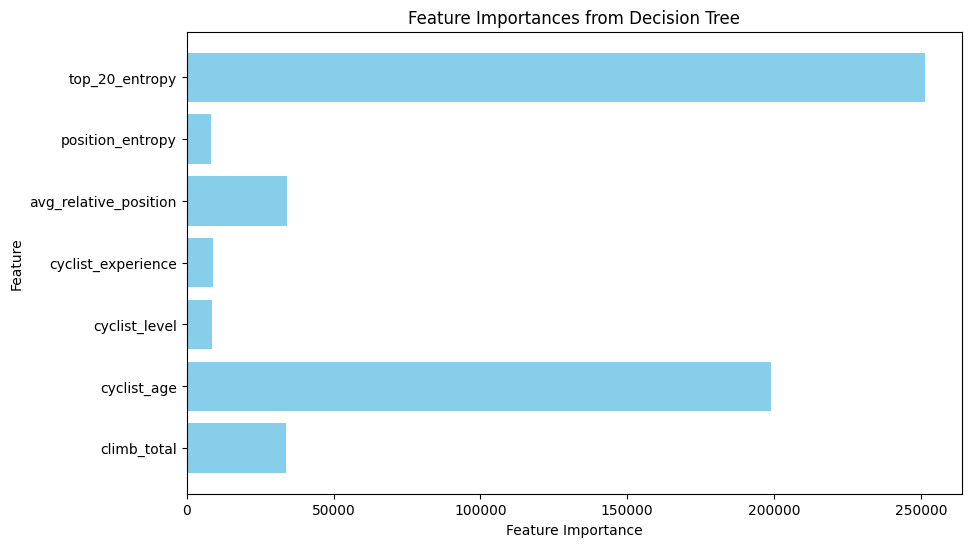
\includegraphics[width=0.4\linewidth]{images/CLASSIFICATION/gmb_feat_import.png}
    \caption{\small Feature importance plot for the GBM Model}
    \label{fig:gbm-feat-importance}
\end{figure}